\documentclass[12pt, titlepage]{article}

\usepackage{fullpage}
\usepackage[round]{natbib}
\usepackage{multirow}
\usepackage{booktabs}
\usepackage{tabularx}
\usepackage{graphicx}
\usepackage{float}
\usepackage{hyperref}
\hypersetup{
    colorlinks,
    citecolor=black,
    filecolor=black,
    linkcolor=red,
    urlcolor=blue
}
\usepackage[round]{natbib}

\newcounter{acnum}
\newcommand{\actheacnum}{AC\theacnum}
\newcommand{\acref}[1]{AC\ref{#1}}

\newcounter{ucnum}
\newcommand{\uctheucnum}{UC\theucnum}
\newcommand{\uref}[1]{UC\ref{#1}}

\newcounter{mnum}
\newcommand{\mthemnum}{M\themnum}
\newcommand{\mref}[1]{M\ref{#1}}

\title{SE 3XA3: Module Guide}

\author{Group \#10
        \\Lab: L03
		\\ Aamina Hussain, hussaa54
		\\ Jessica Dawson, dawsor1
		\\ Fady Morcos, morcof2
}

\date{}

%\input{../../Comments}

\begin{document}

\maketitle

\pagenumbering{roman}
\tableofcontents
\listoftables
\listoffigures

\begin{table}[h!]
\caption{\bf Revision History}
\begin{tabularx}{\textwidth}{p{3cm}p{2cm}X}
\toprule {\bf Date} & {\bf Version} & {\bf Notes}\\
\midrule
March 16, 2022 & 0.0 & Initial Document; Completed Section 3, 7\\
March 17, 2022 & 0.1 & Completed Section 2, 6\\
March 18, 2022 & 0.2 & Completed Section 1, 4, 5\\
\bottomrule
\end{tabularx}
\end{table}

\newpage

\pagenumbering{arabic}

\section{Introduction}

This document is the module guide for the Abstract Art Generator program. This document is intended to be read by:

\begin{itemize}
  \item Designers and Developers
  \item Future project members/maintainers
  \item Stakeholders
\end{itemize}

The \emph{Abstract Art Generator} project is a Python program which uses Pygame and Pygame\_GUI to display a graphical user interface that allows interaction with the user. It generates random abstract art images that may be exported as PNG files. 

Most successful systems are composed of multiple modules, and this modularization allows for better understandability and maintainability. It also creates a simple way to add new features and deal with the anticipated changes without having to re-implement the entire system.

The Python Painters Team made the decision to follow a \emph{Design for Change} design pattern, as well as the concept of information hiding, where each module holds a single secret.

This document will break down the system into modules, each of which will have their own MIS specified in the MIS document. It will also contain a traceability matrix mapping every requirement from the SRS document to at least one of the modules.

The rest of the document is organized as follows. Section
\ref{SecChange} lists the anticipated and unlikely changes of the software
requirements. Section \ref{SecMH} summarizes the module decomposition that
was constructed according to the likely changes. Section \ref{SecConnection}
specifies the connections between the software requirements and the
modules. Section \ref{SecMD} gives a detailed description of the
modules. Section \ref{SecTM} includes two traceability matrices. One checks
the completeness of the design against the requirements provided in the SRS. The
other shows the relation between anticipated changes and the modules. Section
\ref{SecUse} describes the use relation between modules.

\section{Anticipated and Unlikely Changes} \label{SecChange}

This section lists possible changes to the system. According to the likeliness
of the change, the possible changes are classified into two
categories. Anticipated changes are listed in Section \ref{SecAchange}, and
unlikely changes are listed in Section \ref{SecUchange}.

\subsection{Anticipated Changes} \label{SecAchange}

Anticipated changes are the source of the information that is to be hidden
inside the modules. Ideally, changing one of the anticipated changes will only
require changing the one module that hides the associated decision. The approach
adapted here is called design for
change.

\begin{description}
\item[\refstepcounter{acnum} \actheacnum \label{acLayerDraw}:] The ways layers can be drawn, new or modified drawing algorithms.
\item[\refstepcounter{acnum} \actheacnum \label{acWidget}:] What widgets exist.
\item[\refstepcounter{acnum} \actheacnum \label{acUILayout}:] The layout of the UI.
\item[\refstepcounter{acnum} \actheacnum \label{acHelp}:] The contents of the help dialogue.
\item[\refstepcounter{acnum} \actheacnum \label{acPalettes}:] The list of color palettes.
\end{description}

\subsection{Unlikely Changes} \label{SecUchange}

The module design should be as general as possible. However, a general system is
more complex. Sometimes this complexity is not necessary. Fixing some design
decisions at the system architecture stage can simplify the software design. If
these decision should later need to be changed, then many parts of the design
will potentially need to be modified. Hence, it is not intended that these
decisions will be changed.

\begin{description}
\item[\refstepcounter{ucnum} \uctheucnum \label{ucIO}:] The library used for input and graphical display.
\item[\refstepcounter{ucnum} \uctheucnum \label{ucPalette}:] The existence of the color palette widget.
\end{description}

\section{Module Hierarchy} \label{SecMH}

%Each one of the setting dialogues on the UI is defined as a widget which handles behaviour relating to it, the color palette is a widget, each of the layers is a widget, etc.

This section provides an overview of the module design. Modules are summarized
in a hierarchy decomposed by secrets in Table \ref{TblMH}. The modules listed
below, which are leaves in the hierarchy tree, are the modules that will
actually be implemented.

\begin{description}
\item [\refstepcounter{mnum} \mthemnum \label{mHH}:] Hardware-Hiding Module
\item [\refstepcounter{mnum} \mthemnum \label{mUI}:] Controller UI Module
\item [\refstepcounter{mnum} \mthemnum \label{mCV}:] Canvas Module
\item [\refstepcounter{mnum} \mthemnum \label{mW}:] Widget Module
\item [\refstepcounter{mnum} \mthemnum \label{mL}:] Layer Module
\item [\refstepcounter{mnum} \mthemnum \label{mOL}:] Overlay Module
\item [\refstepcounter{mnum} \mthemnum \label{mCP}:] Color Palette Module
\item [\refstepcounter{mnum} \mthemnum \label{mH}:] Help Module
\item [\refstepcounter{mnum} \mthemnum \label{mGS}:] Generate Shape Module
\item [\refstepcounter{mnum} \mthemnum \label{mWS}:] Widget Storage Module
\item [\refstepcounter{mnum} \mthemnum \label{mA}:] Assets Module
\end{description}


\begin{table}[h!]
\centering
\begin{tabular}{p{0.3\textwidth} p{0.6\textwidth}}
\toprule
\textbf{Level 1} & \textbf{Level 2}\\
\midrule

{Hardware-Hiding Module} & pygame Library \\
\midrule

\multirow{1}{0.3\textwidth}{Behaviour-Hiding Module} & Controller UI Module\\
\midrule

\multirow{9}{0.3\textwidth}{Software Decision Module} & Canvas Module\\
& Widget Module\\
& Layer Module\\
& Overlay Module\\
& Color Palette Module\\
& Help Module\\
& Generate Shape Module\\
& Widget Storage Module\\
& Assets Module\\
\bottomrule

\end{tabular}
\caption{Module Hierarchy}
\label{TblMH}
\end{table}

\newpage
\section{Connection Between Requirements and Design} \label{SecConnection}

The design of the system is intended to satisfy the requirements developed in
the SRS. In this stage, the system is decomposed into modules. The connection
between requirements and modules is listed in Table \ref{TblRT} which is located in section 7 of this document. However readers of this document are recommended to read section 3 and section 5 first before looking at the traceability matrix in section 7.

\section{Module Decomposition} \label{SecMD}

Modules are decomposed according to the principle of ``information hiding''
proposed by \citet{ParnasEtAl1984}. The \emph{Secrets} field in a module
decomposition is a brief statement of the design decision hidden by the
module. The \emph{Services} field specifies \emph{what} the module will do
without documenting \emph{how} to do it. For each module, a suggestion for the
implementing software is given under the \emph{Implemented By} title. If the
entry is \emph{OS}, this means that the module is provided by the operating
system or by standard programming language libraries.  Also indicate if the
module will be implemented specifically for the software.

Only the leaf modules in the
hierarchy have to be implemented. If a dash (\emph{--}) is shown, this means
that the module is not a leaf and will not have to be implemented. Whether or
not this module is implemented depends on the programming language
selected.

\subsection{Hardware Hiding Modules (\mref{mHH})}

\begin{description}
\item[Secrets:]The data structure and algorithm used to implement the virtual
  hardware.
\item[Services:]Serves as a virtual hardware used by the rest of the
  system. This module provides the interface between the hardware and the
  software. So, the system can use it to display outputs or to accept inputs.
\item[Implemented By:] pygame
\end{description}

\subsection{Behaviour-Hiding Module}

\begin{description}
\item[Secrets:]The contents of the required behaviours.
\item[Services:]Includes programs that provide externally visible behaviour of
  the system as specified in the software requirements specification (SRS)
  documents. This module serves as a communication layer between the
  hardware-hiding module and the software decision module. The programs in this
  module will need to change if there are changes in the SRS.
\item[Implemented By:] N/A
\end{description}

\subsubsection{Controller UI Module (\mref{mUI})}

\begin{description}
\item[Secrets:] The processes required to convert user input into a display.
\item[Services:] Takes in input data from the user and displays corresponding visual output.
\item[Implemented By:] AbstractArtGenerator
\end{description}


\subsection{Software Decision Module}

\begin{description}
\item[Secrets:] The design decision based on mathematical theorems, physical
  facts, or programming considerations. The secrets of this module are
  \emph{not} described in the SRS.
\item[Services:] Includes data structure and algorithms used in the system that
  do not provide direct interaction with the user. 
  % Changes in these modules are more likely to be motivated by a desire to
  % improve performance than by externally imposed changes.
\item[Implemented By:] N/A
\end{description}

\subsubsection{Canvas Module (\mref{mCV})}

\begin{description}
\item[Secrets:] The decision making for how the pygame surfaces are placed in the display.
\item[Services:] Includes the main decision making for how the art image is produced.
\item[Implemented By:] AbstractArtGenerator
\end{description}

\subsubsection{Widget Module (\mref{mW})}

\begin{description}
\item[Secrets:] The abstract methods other classes can inherit.
\item[Services:] An abstract class that contains a framework of methods other classes can inherit and use. This accounts for anticipated changes.
\item[Implemented By:] AbstractArtGenerator
\end{description}

\subsubsection{Layer Module (\mref{mL})}

\begin{description}
\item[Secrets:] The processes required to generate a layer.
\item[Services:] Contains all methods relating to generating, displaying, and interacting with the layers of the generated art image.
\item[Implemented By:] AbstractArtGenerator
\end{description}

\subsubsection{Overlay Module (\mref{mOL})}

\begin{description}
\item[Secrets:] The processes required to use an overlay/border.
\item[Services:] Contains all methods relating to displaying and interacting with the overlays/borders that are placed over top of the generated art image.
\item[Implemented By:] AbstractArtGenerator
\end{description}

\subsubsection{Color Palette Module (\mref{mCP})}

\begin{description}
\item[Secrets:] The processes required to use the color palettes.
\item[Services:] Contains all methods relating to displaying, randomly choosing, and interacting with the color palette options.
\item[Implemented By:] AbstractArtGenerator
\end{description}

\subsubsection{Help Module (\mref{mH})}

\begin{description}
\item[Secrets:] How the instructions are displayed.
\item[Services:] Contains all methods relating to displaying the instructions and interacting with the help option.
\item[Implemented By:] AbstractArtGenerator
\end{description}

\subsubsection{Generate Shape Module (\mref{mGS})}

\begin{description}
\item[Secrets:] The processes required to generate shapes.
\item[Services:] Contains methods that are used to generate different shapes that are a part of each layer of the art image.
\item[Implemented By:] AbstractArtGenerator
\end{description}

\subsubsection{Widget Storage Module (\mref{mWS})}

\begin{description}
\item[Secrets:] Storage for program widgets.
\item[Services:] Allows all other modules to access \texttt{program widgets}. The widgets include the layer module, help module, overlay module, and color palette module.
\item[Implemented By:] AbstractArtGenerator
\end{description}

\subsubsection{Assets Module (\mref{mA})}

\begin{description}
\item[Secrets:] Storage for assets (such as constants).
\item[Services:] Contains assets that are used by other modules.
\item[Implemented By:] AbstractArtGenerator
\end{description}

\section{Traceability Matrix} \label{SecTM}

This section shows two traceability matrices: between the modules and the
requirements and between the modules and the anticipated changes.

% the table should use mref, the requirements should be named, use something
% like fref
\begin{table}[H]
\centering
\begin{tabular}{p{0.2\textwidth} p{0.6\textwidth}}
\toprule
\textbf{Req.} & \textbf{Modules}\\
\midrule
FR1 & \mref{mCP}\\
FR2 & \mref{mUI}, \mref{mCP}\\
FR3 & \mref{mUI}, \mref{mCV}\\
FR4 & \mref{mL}, \mref{mGS}\\
FR5 & \mref{mUI}, \mref{mL}\\
FR6 & \mref{mCV}\\
FR7 & \mref{mUI}, \mref{mCV}, \mref{mA}\\
FR8 & \mref{mUI}, \mref{mCV}, \mref{mA}\\
FR9 & \mref{mUI}, \mref{mCV}, \mref{mA}\\
FR10 & \mref{mUI}, \mref{mCV}, \mref{mOL}\\
FR11 & \mref{mUI}, \mref{mOL}\\
FR12 & \mref{mUI}, \mref{mH}, \mref{mA}\\
FR13 & \mref{mUI}\\
LF1 & \mref{mCV}, \mref{mL}, \mref{mOL}, \mref{mCP}\\
LF2 & \mref{mCV}\\
UH1 & \mref{mUI}, \mref{mCV}\\
UH2 & \mref{mUI}, \mref{mL}, \mref{mOL}, \mref{mCP}, \mref{mH}, \mref{mA}\\
UH3 & \mref{mUI}, \mref{mH}\\
PR1 & \mref{mUI}\\
PR2 & \mref{mCV}\\
\bottomrule
\end{tabular}
\caption{Trace Between Requirements and Modules}
\label{TblRT}
\end{table}

\begin{table}[H]
\centering
\begin{tabular}{p{0.2\textwidth} p{0.6\textwidth}}
\toprule
\textbf{AC} & \textbf{Modules}\\
\midrule
\acref{acLayerDraw} & \mref{mL}, \mref{mOL}, \mref{mGS}\\
\acref{acWidget} & \mref{mUI}, \mref{mWS}\\
\acref{acUILayout} & \mref{mUI}\\
\acref{acHelp} & \mref{mH}\\
\acref{acPalettes} & \mref{mCP}\\
\bottomrule
\end{tabular}
\caption{Trace Between Anticipated Changes and Modules}
\label{TblACT}
\end{table}


% \item [\refstepcounter{mnum} \mthemnum \label{mHH}:] Hardware-Hiding Module
% \item [\refstepcounter{mnum} \mthemnum \label{mUI}:] Controller UI Module
% \item [\refstepcounter{mnum} \mthemnum \label{mCV}:] Canvas Module
% \item [\refstepcounter{mnum} \mthemnum \label{mW}:] Widget Module
% \item [\refstepcounter{mnum} \mthemnum \label{mL}:] Layer Module
% \item [\refstepcounter{mnum} \mthemnum \label{mOL}:] Overlay Module
% \item [\refstepcounter{mnum} \mthemnum \label{mCP}:] Color Palette Module
% \item [\refstepcounter{mnum} \mthemnum \label{mH}:] Help Module
% \item [\refstepcounter{mnum} \mthemnum \label{mGS}:] Generate Shape Module
% \item [\refstepcounter{mnum} \mthemnum \label{mMS}:] Widget Storage Module
% \item [\refstepcounter{mnum} \mthemnum \label{mA}:] Assets Module


\section{Use Hierarchy Between Modules} \label{SecUse}

In this section, the uses hierarchy between modules is
provided.

\begin{figure}[H]
\centering
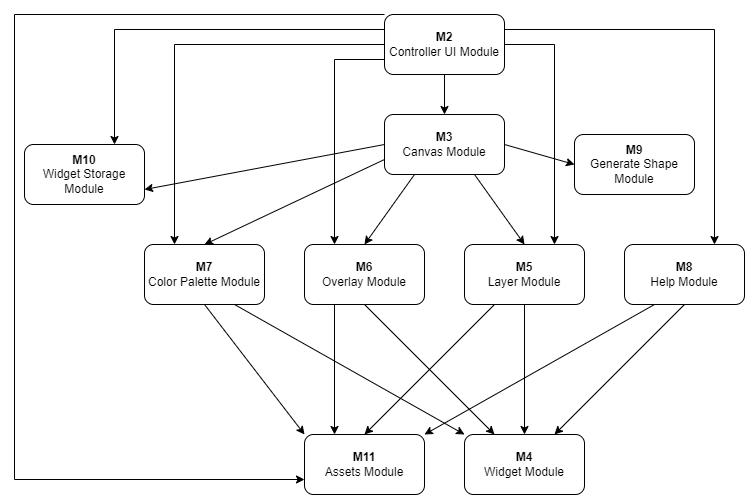
\includegraphics[width=0.7\textwidth]{images/UsesHierarchy.png}
\caption{Use hierarchy among modules}
\label{FigUH}
\end{figure}

%\section*{References}

\bibliographystyle {plainnat}
\bibliography {MG}

\end{document}
